
\section{Modelling of \texorpdfstring{\nb}{Nb} templates with loose and tight working points}
\label{sec:nb_validation}

Likelihood-based \nb validation, as described in Section~\ref{sec:nb-zinv}, are repeated also using \mmj sample, 
with loose and tight working point respectively, to check consistency between \nb modelling in b-jet enriched and 
mistag enriched environments. The results are shown in Figure~\ref{fig:loose_tight_nb}.

\begin{figure}[h!]
  \centering
  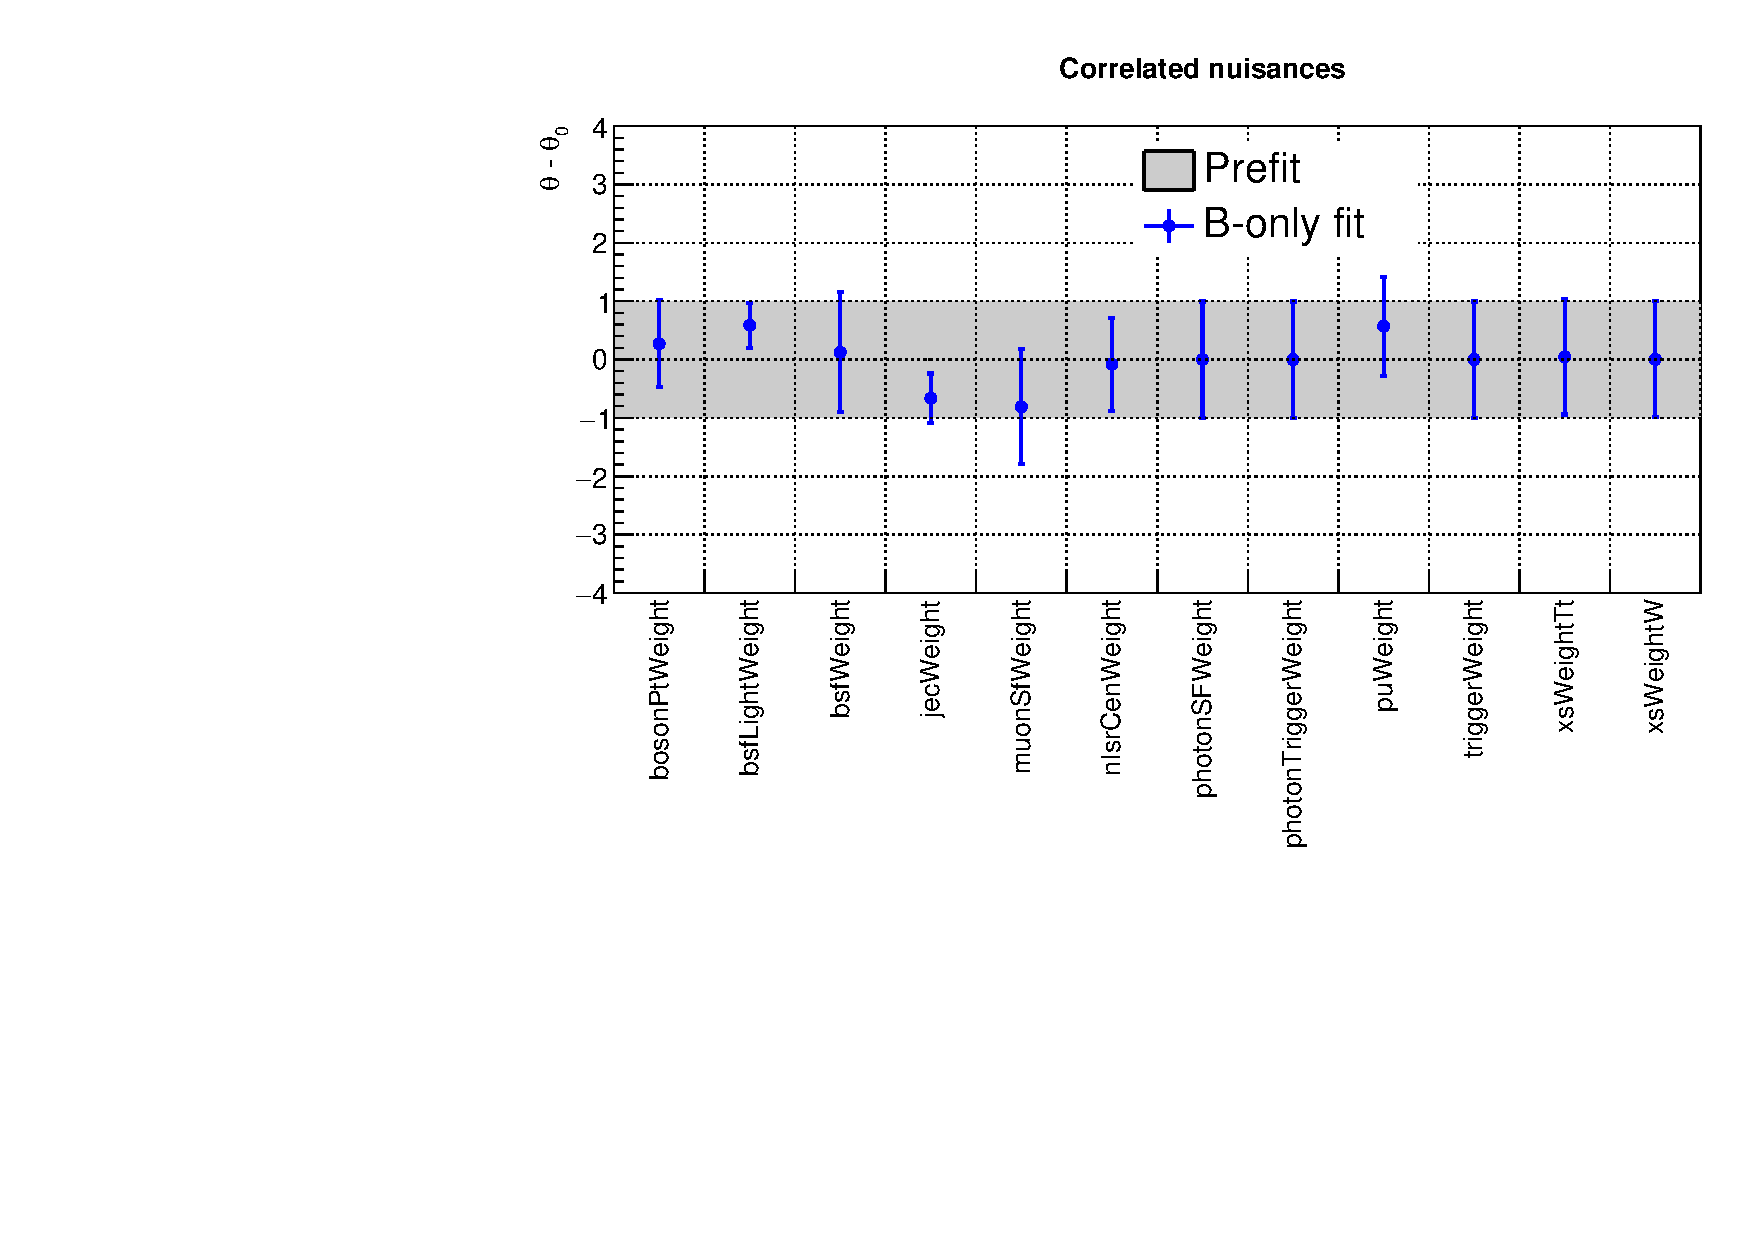
\includegraphics[width=0.6\textwidth]{figures/btag/nuisances/full/Correlated_nuisances_loose}
  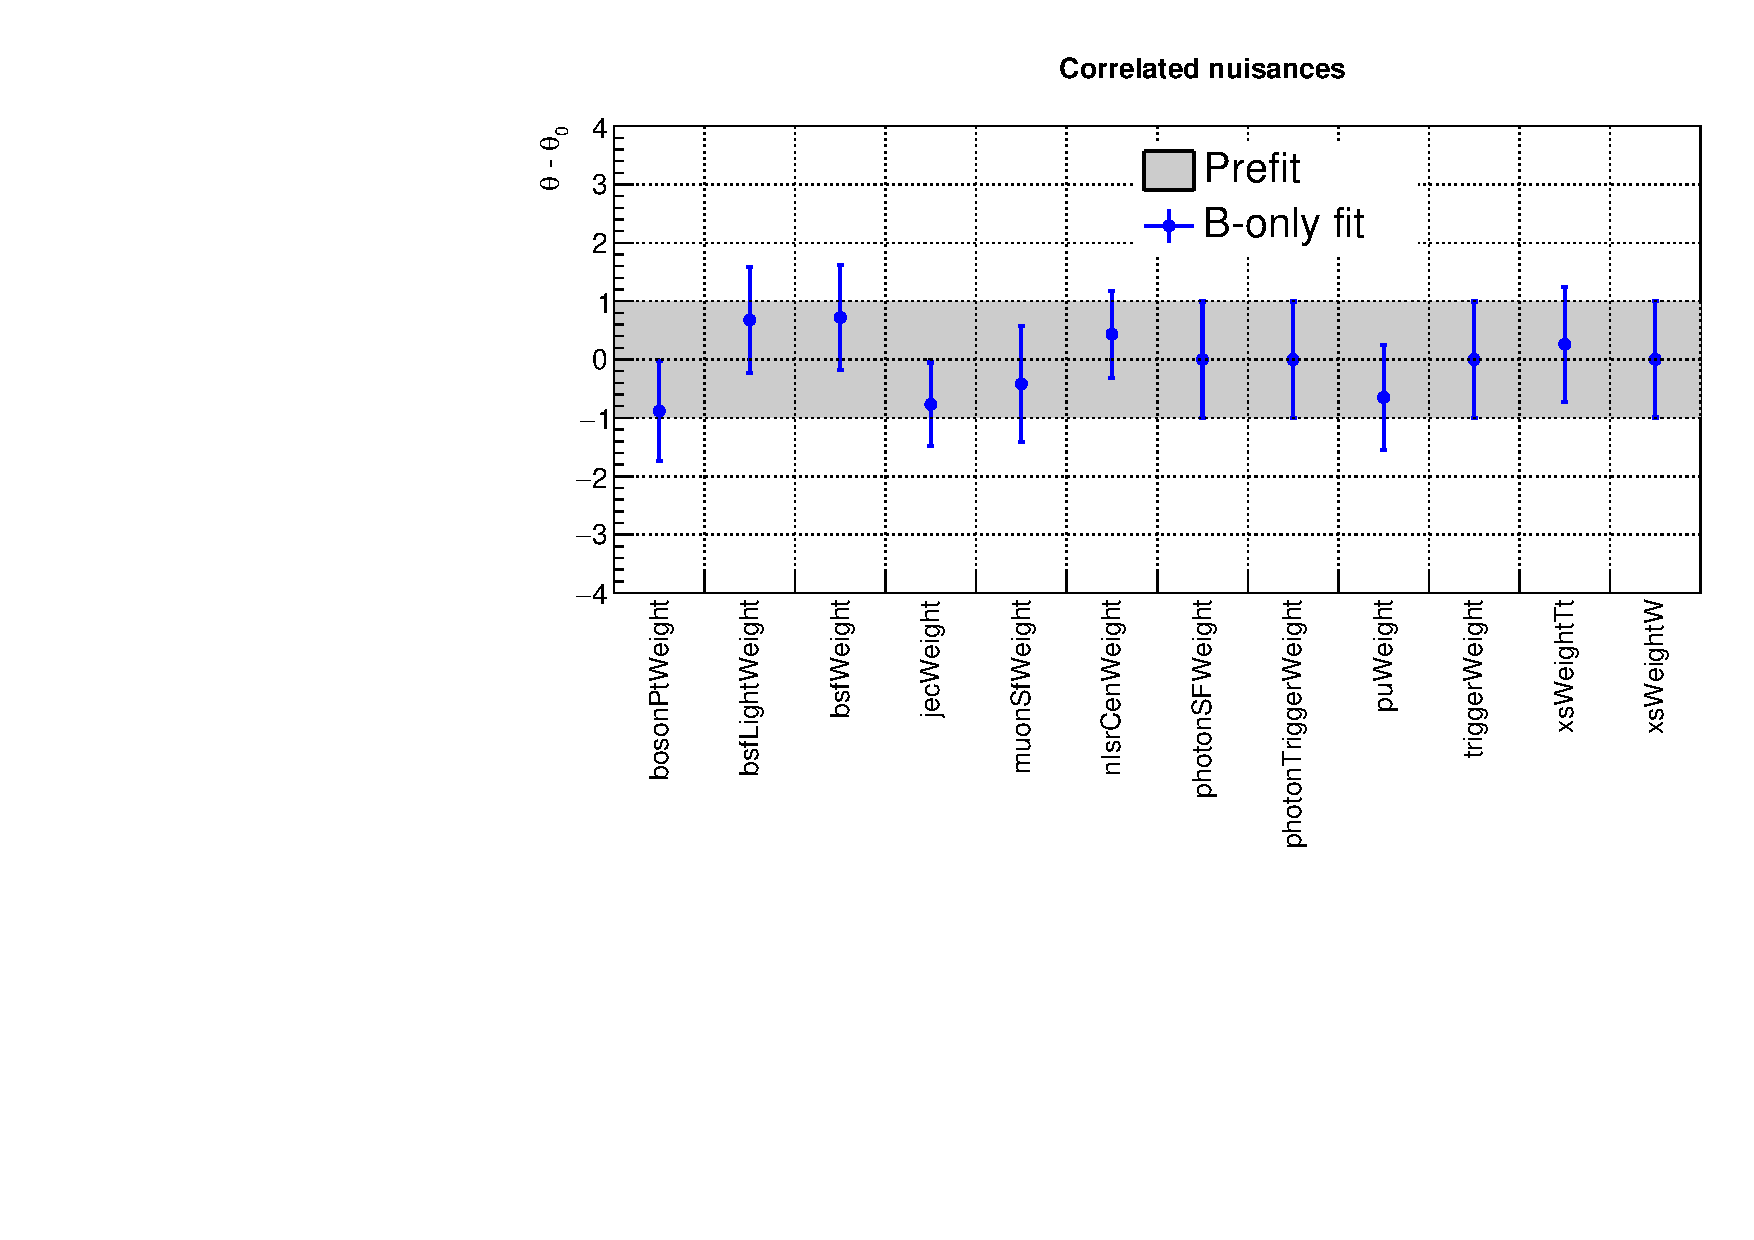
\includegraphics[width=0.6\textwidth]{figures/btag/nuisances/full/Correlated_nuisances_tight}
  \caption{\label{fig:btagsfge1b} Post-fit nuisances of a likelihood
    fit to data in the \mmj control region with loose (top) and tight (bottom)
    btagging working points. }
  \label{fig:loose_tight_nb}
\end{figure}

